\documentclass[a4paper]{article}

%use the english line for english reports
%usepackage[english]{babel}
\usepackage[portuguese]{babel}
\usepackage[utf8]{inputenc}
\usepackage{indentfirst}
\usepackage{graphicx}
\usepackage{verbatim}
\usepackage{mathtools}
\usepackage{amsmath}
\usepackage[export]{adjustbox}


\begin{document}

\setlength{\textwidth}{16cm}
\setlength{\textheight}{22cm}

\title{\Huge\textbf{Otimização da Gestão de Projetos}\linebreak\linebreak\linebreak
\Large\textbf{Relatório Final}\linebreak\linebreak
\linebreak\linebreak

\includegraphics[scale=0.1]{feup-logo.png}\linebreak\linebreak
\linebreak\linebreak
\Large{Mestrado Integrado em Engenharia Informática e Computação} \linebreak\linebreak
\Large{Inteligência Artificial}\linebreak
}

\author{\textbf{Grupo B5.3:}\\ André Costa Moreira Maia - 201200674 - up201200674@fe.up.pt \\ Guilherme Vieira Pinto - 201305803 - up201305803@fe.up.pt \\ João Manuel Estrada Pereira Gouveia - 201303988 - up201303988@fe.up.pt \\ \linebreak\linebreak \\
 \\ Faculdade de Engenharia da Universidade do Porto \\ Rua Roberto Frias, s\/n, 4200-465 Porto, Portugal \linebreak\linebreak\linebreak
\linebreak\linebreak\vspace{1cm}}
%\date{Junho de 2007}
\maketitle
\thispagestyle{empty}

%************************************************************************************************
%************************************************************************************************

\newpage

\section*{Objetivo}

Este trabalho é desenvolvido no âmbito da unidade curricular de Inteligência Artificial (IART), e tem como principal objectivo o estudo e investigação de algoritmos de otimização de soluções. \\ No projeto em questão, será abordada a otimização da gestão de projetos, isto é, a distribuição de trabalhadores pelas tarefas de um determinado projeto. Sendo que esta atribuição ocupa um vasto campo de soluções para projetos complexos com um considerável número de trabalhadores, recorremos a metodologias de otimização de soluções como algoritmos genéticos e arrefecimento simulado para alcançar o objectivo pretendido.

 \par Tendo em conta a complexidade da organização de recursos orientados à gestão de projetos coordenados, temos como objetivo, o output de um valor ótimo para o problema.  
 
 \par Definiremos então um Projeto como sendo constituído por uym conjunto de Tarefas a serem concluídas por um ou mais Trabalhadores. As Tarefas podem ter precedências entre si e apresentam uma duração Trabalhador/mês. Cada tarefa não pode ser iniciada sem a totalidade das suas precedências estar completa.
 


\newpage

\tableofcontents

%************************************************************************************************
%************************************************************************************************

%*************************************************************************************************
%************************************************************************************************

\newpage

%%%%%%%%%%%%%%%%%%%%%%%%%%
\section{Especificação}
O problema apresentado enquadra-se no paradigma da otimização de projetos generalizados. 
\paragraph{}
Tendo em conta as variáveis a ser trabalhadas, devemos ter em conta os seguintes pontos:
\begin{itemize}
	\item Um \textit{Projeto} é constituido por uma ou mais \textit{Tarefas};
	\item Uma \textit{Tarefa} tem associadas as seguintes carateristicas:
	\begin{itemize}
		\item Duração (Pessoas/Mês);
		\item \textit{Tarefas} precedentes;
		\item \textit{Scope} (Âmbito);
	\end{itemize}
	\item Um \textit{Trabalhador} é caracterizado pelas suas \textit{Skills} (Competências);
	\item Uma \textit{Skill} é constituída pelo tuplo \textit{Scope}-\textit{Performance}.
\end{itemize}

Relativamente a algumas definições dos termos acima mencionados, deve-se clarificar os seguintes:
\begin{itemize}
	\item \textbf{Duração do Projeto} - O término do projeto deverá corresponder ao final da execução da última tarefa concluida;
	\item \textbf{Execução de uma Tarefa} - Uma tarefa só deve ser iniciada quando todas as suas precedências foram concluidas;
	\item \textbf{Duração em Pessoa/Mês} - Esta unidade de tempo foi interpretada de forma a que, dada uma tarefa com \textit{Scope} \textbf{S}, com duração de \textbf{t} Pessoas/Mês e tendo a ela associados \textbf{n} trabalhadores com um somatório total de \textbf{P} \textit{Performance} (sendo que apenas as performances consideradas são relativas a \textit{Skills} equivalentes a \textbf{S}), temos: \textbf{\textit{RealDuration} = $\frac{t}{P}$}, sendo \textit{RealDuration}, a duração definitiva da Tarefa após atribuição dos Trabalhadores;
	\item \textbf{Atribuição de Trabalhadores} - Na nossa abordagem, é possivel a atribuição de Trabalhadores a Tarefas cujas \textit{Skills} não se enquadrem na \textit{Scope} pretendida; no entanto, estes Trabalhadores em nada influenciarão o progresso da Tarefa;
\end{itemize}
Os resultados obtidos na execução do programa fornecerão uma solução otimizada para uma alocação eficaz de elementos de uma equipa de Trabalhadores, avaliando as diversas fases de desenvolvimento de um Projeto e, tendo em conta a possivel escalabilidade do caso para situações de maior porte, é possivel considerar a sua aplicação num enquadramento empresarial.
\newpage

Para este problema, serão aplicados algoritmos orientados para a resolução de problemas de otimização, sendo eles Algoritmos Genéticos e Arrefecimento Simulado tendo em conta que a sua natureza probabilística permite o alcance e seleção de soluções aceitáveis sem ter que considerar todo o campo de hipóteses.

\subsection{Algoritmos Genéticos}
Os Algoritmos Genéticos pertencem à classe de algoritmos evolutivos, recorrendo a métodos de simulação comportamental de uma população de forma a que a seleção de soluções boas geram soluções progressivamente melhores. Para tal, são adotadas técnicas inspiradas na biologia evolutiva como mutação, seleção e reprodução (\textit{crossover}).
\paragraph{}
Na nossa abordagem ao algoritmo, começamos pela definição da representação dos cromossomas a serem processados.
\paragraph{}
\begin{figure}[!ht]
	\centering
	\includegraphics[scale=0.5]{chromosome.png}
	\caption{Representação de um cromossoma esquematizando um projeto constituído por três tarefas e seis trabalhadores associados.}
\end{figure}
\paragraph{Cromossomas}Os cromossomas planeados serão estruturados como arrays binários com dimensão \textit{T$\times$W} (sendo que T simboliza o número de tarefas do projeto e W o número de trabalhadores a ele associados). O cromossoma representa, portanto, o projeto na íntegra, na medida em que inclui cada tarefa que o constitui. Esta representação permite identificar que trabalhadores estão associados para cada tarefa, sendo que o valor 1 num bit indica que o respetivo trabalhador lhe está destacado. Esta análise é explicada mais detalhadamente no cálculo de \textit{fitness} de cada cromossoma.
\paragraph{Variáveis}
Ao iniciar o algoritmo, uma população com um determinado número de cromossomas é gerado. É definido o número de gerações a serem executadas, o número de cortes por cromossoma durante o \textit{crossover} e a respetiva probabilidade de mutação na criação de um novo cromossoma dele derivado. É também possível definir o número de seleções por geração, caso se pretenda que o algoritmo opte por uma metodologia de seleção elitista ou, caso contrário, este adotará o método de seleção probabilistico, tendo em conta os \textit{fitness's} da população.
\paragraph{População}
No decorrer do algoritmo, à medida que novas gerações são geradas, determinados indivíduos são excluidos para a próxima iteração, quer por motivos de penalização por \textit{fitness} insatisfatório ou por seleção. De modo a preencher a população da geração seguinte, por cada elementos excluído, são gerados novos cromossomas por \textit{crossover}, mantendo a integridade do domínio de soluções.
\newpage
\paragraph{Seleção}
Na seleção de individuos de uma população, devemos ter em conta o tipo de análise a ser feita. Para tal, o array de cromossomas deve ser constantemente ordenado de geração para geração, por ordem crescente de \textit{fitness}, e com os individuos de \textit{fitness} negativo no final do array. Caso o número de seleções seja especificado, o método de escolha será elitista: sendo \textit{N} o número de seleções pretendidas, o array ordenado de cromossomas é percorrido apartir do primeiro índice, até à posição \textit{N-1}, eliminando todos os cromossomas com \textit{fitness} negativo e aqueles que se encontrem apartir da posição de índice \textit{N}, pelo que o array terminará sempre com um máximo de N elementos. Caso contrário, se o número elementos a selecionar não seja especificado, apenas os cromossomas com \textit{fitness} negativo serão excluídos.
\paragraph{Crossover}
Relativamente ao \textit{crossover}, este será executado tantas vezes quantas forem necessárias para completar a população, de modo a preencher as vagas geradas durante a seleção. Para tal, é preciso considerar se o algoritmo genétio está ser executado segundo uma prespetiva elitista ou não. Avaliando se o número de selecoes foi especificado: se foi, então são selecionados os 2 melhores cromossomas para \textit{crossover}, caso contrário, são avaliados todos os cromossomas ainda presentes na população tendo em conta os seus \textit{fitnesses} e, quanto melhor o seu valor, mais probabilidade terão de ser selecionados para \textit{crossover}. Para além da determinação de cromossomas, é preciso tb o processamento de cortes: tendo em conta o número de cortes especificado, serão gerados índices de corte distintos de modo a determinar o ponto de \textit{crossover} entre os cromossomas elegidos.
\paragraph{}
\begin{figure}[!ht]
	\centering
	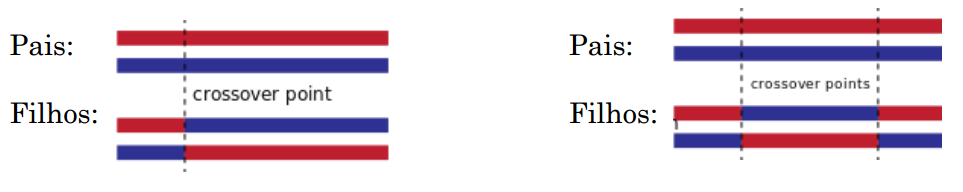
\includegraphics[scale=0.5]{crossover.png}
	\caption{Representação do processo de crossover para uma situação com um corte (esquerda) ou dois cortes (direita)}
\end{figure}
\paragraph{Mutação}
Cada cromossoma resultante de um \textit{crossover} terá os seus genes percorridos de modo a executar um sorteio de mutação para cada bit, tendo em conta a probabilidade de mutação definida. Caso seja definida mutação num determinado índice, o respetivo bit é modificado para o valor oposto.
\paragraph{\textit{Fitness}}
A definição da função de \textit{fitness} é o ponto crucial deste algoritmo, pelo que quantificará cada cromossoma e influenciará diretamente o decorrer da evolução da população a cada geração processada.
\paragraph{}
O valor de \textit{fitness} calculado corresponderá ao valor do tempo de execução do projeto, caso a representação do cromossoma constitua uma alocação de trabalhadores válida para a a sua execução, caso contrário será quantificado como -1. Mais especificamente, entende-se como "válida", a alocação de trabalhadores tal que, para uma dada tarefa com \textit{Scope} \textbf{S}, exista pelo menos um trabalhador a ela destacado que possua uma \textit{Skill} compatível a \textbf{S}.
\paragraph{}
A determinação do tempo de execução de um projeto será equivalente ao momento de conclusão da última tarefa realizada, pelo que será esse mesmo valor que deveremos avaliar. Para tal, após verificar se a alocação de trabalhadores no cromossoma é válida, procede-se ao calculo da duração de cada tarefa, tendo em conta a execução das suas precedências e a disponibilidade de cada trabalhador a ela destacado.
\paragraph{}
O processamento deste cálculo efetua-se segundo as seguintes fases:
\begin{itemize}
	\item Iniciar loop com \textbf{T} iterações, sendo \textbf{T}, o número de tarefas que constituem o projeto;
	\item Para cada iteração, percorrer \textbf{W} indices do cromossoma, sendo \textbf{W} o número de trabalhadores criados para o projeto;
	\item Para cada indice percorrido, caso o bit esteja assinalado com o valor "1", consultar os dados do trabalhador que lhe é respetivo, determinando se este possui alguma competência para influenciar o desenvolvimento da tarefa, acumulando a respetiva performance à performance total dedicada por todos os trabalhadores destacados à tarefa;
	\item Após reunir a informação relativa à performance total, determinar o tempo de inicio de execução da tarefa. Sendo que o tempo de início de execução de uma tarefa corresponde ao momento de finalização de todas as suas precedências, e tendo em conta que as tarefas são analisadas por ordem cronológica (não existe nenhuma situação em que uma dada tarefa seja processada antes das suas precedências), conseguimos obter facilmente este valor;
	\item Calcular o tempo de execução, sendo este determinado pela fórmula enunciada na página 4, ao clarificar a definição de duração de uma tarefa;
	\item Obtendo os resultados dos últimos dois pontos, é-nos possivel determinar o momento de finalização da tarefa a ser analizada na iteração atual;
	\item Finalmente, deve-se atualizar os dados dos trabalhadores relativos à disponibilidade de cada um e armazenando o tempo de finalização desta tarefa.
\end{itemize}
\paragraph{}
Após execução das instruções acima enunciadas, obtém-se uma lista de resultados relativa ao momento de finalização de cada tarefa. O valor de \textit{fitness} que pretendemos obter consiste no máximo presente nesta lista.
\paragraph{}
Sendo que o objetivo do problema é determinar a melhor forma para diminuir o tempo de execução de um projeto, o cromossoma mais Apto será aquele que apresentar menor \textit{fitness}.
\newpage

\subsection{Arrefecimento Simulado}
\paragraph{}
O Arrefecimento Simulado (\textit{Simulated Annealing}) consiste numa meta-heurística para otimização de problemas onde recorre a técnicas de busca local probabilística//aleatória, fundamentando-se numa analogia relacionada com termodinâmica. O processo denominado de \textit{annealing} é utilizado na metalurgia e consiste no aumento de um metal, seguido de um arrefecimento lento e controlado, de modo a atingir-se um estado energético baixo o suficiente para garantir uma menor energia interna, reduzindo possiveis defeitos do resultado.
\paragraph{}
Na nossa abordagem ao problema, decidimos optar por uma adaptação dos calculos executados nos algoritmos genéticos, modificando-os de forma a que se enquadrassem no processamento deste algoritmo em específico. Mais concretamente, o codigo reutilizado consiste no cálculo do valor do estado atual: recorrendo ao mesmo processo de análise do tempo de execução de um projeto no Algoritmo Genético, executamos as mesmas operações. Contudo, existem pequenas alterações relativamente à penalização. Uma vez que pretendemos sempre avançar num sentido que favoreça, de modo individual, um determinado estado, convém nao generalizar os casos em que um projeto não pode ser concluido. Sendo assim, para cada tarefa que não possa ser concluida, por não ter trabalhadores aptos para a executar, acrescenta-se a penalização de dez meses acrescidos à duraçao original do projeto. Esta análise de cada estado torna-se simples na medida em que a representação do conhecimento é igual à representação dos cromossomas, nos Algoritmos Genéticos.
\paragraph{}
O algoritmo depende de duas variavéis: a temperatura e o rácio de diminuição da temperatura. Ambos os valores poderão ser especificados pelo utilizador, de modo a ser possivel retirar conclusões mais claras relativamente à eficácia do algoritmo. De acordo com a teoria, quanto maior a temperatura e/ou menor o rácio de diminuição, melhores serão os resultados obtidos.
\paragraph{}
Enquanto a Temperatura \textbf{T} não for igual a 0, o algoritmo encontrar-se-à num loop constante, onde T variará no sentido decrescente, dependendo do rácio estabelecido. A cada iteração, um novo estado \textbf{N}, diferente do atual \textbf{A}, é gerado e avaliado. É, de seguida, calculada a diferença entre os dois estados, tendo que $\bigtriangleup \textrm{E} = \textrm{N} - \textrm{A}$. Tendo este cálculo determinado, definimos que:
\paragraph{}
\[
\begin{cases}
\textrm{A} = \textrm{N}      & \quad \text{if } \bigtriangleup \textrm{E} > 0\\
	\begin{cases}
	\textrm{A} = \textrm{A}     & \quad \text{if } \textrm{Math.random()} > \mathrm{e}^{\frac{\bigtriangleup \textrm{E}}{T}}\\
	\textrm{A} = \textrm{N}  	& \quad \text{if } \textrm{Math.random()} < \mathrm{e}^{\frac{\bigtriangleup \textrm{E}}{T}}\\
	\end{cases}
\end{cases}
\]
\paragraph{}
Tendo em conta o cálculo de $\bigtriangleup \textrm{E}$, não podemos quantificar cada estado como nos Algoritmos Genéticos, pelo que, para definir que um estado é melhor que o outro quando o seu valor é superior, decidimos pela atribuição do valor equivalente a $\mathrm{(\frac{projectDuration}{\textrm{fitness}})}^2$, pelo que \textit{fitnesses} mais elevados, gerarão valores mais baixos, e vice-versa
%%%%%%%%%%%%%%%%%%%%%%%%%%
\newpage
\section{Desenvolvimento}
 Para a implementação deste projeto, recorreremos à linguagem Java que, para além de nos facultar a documentação e estruturas de dados mais importantes para a conceção do código, também suporta, de forma consistente e relativamente simples, a criação de uma interface gráfica importante para a comunicação com o utilizador, de modo a que este possa manipular as variáveis.
\paragraph{} 
A nível de Ferramentas/APIs utilizadas neste projeto, são de referir o Eclipse (usado na elaboração do código), Github (usado um repositório para partilha de código) e TexStudio (usado na elaboração do relatório).
\paragraph{}
Relativamente à GUI, recorremos à biblioteca Swing de Java para estruturar uma interação muito simplificada para receber os inputs pretendidos pelo utilizador.
\paragraph{} 
A seguir demonstra-se o diagrama de classes do referido projeto.
\begin{figure}[!ht]
	\centering
	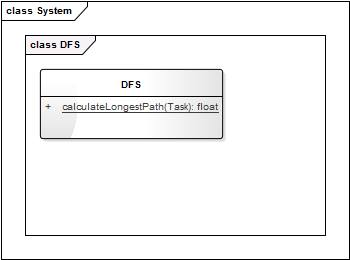
\includegraphics[scale=0.4]{uml1.png}
	\caption{Pacote auxiliar para calculo da duraçao original do projeto}
\end{figure}
\begin{figure}
	\centering
	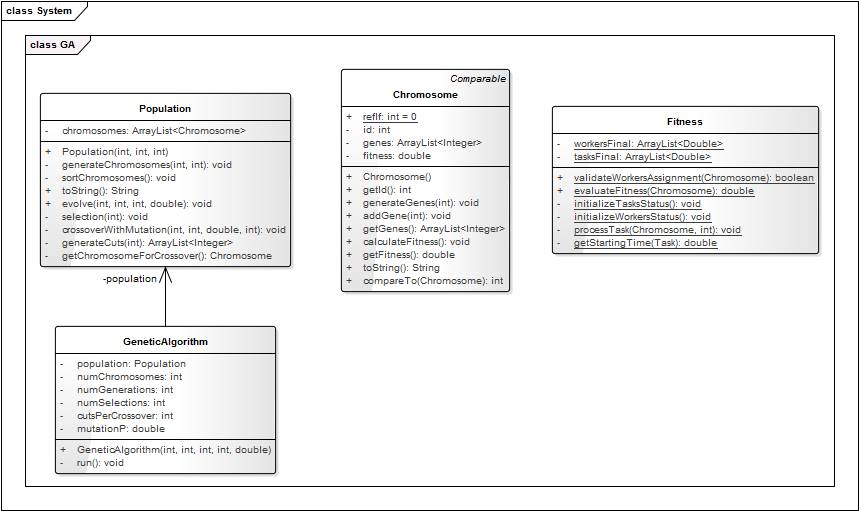
\includegraphics[scale=0.4]{uml2.png}
	\caption{Pacote de Algoritmos Geneticos}
\end{figure}
\begin{figure}
	\centering
	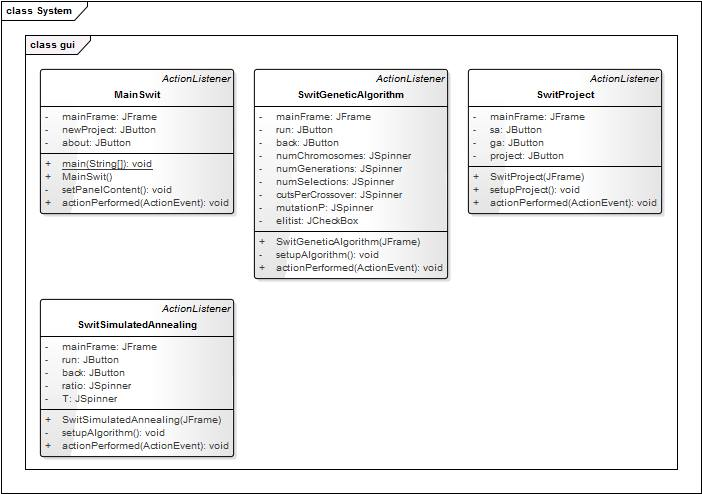
\includegraphics[scale=0.4]{uml3.png}
	\caption{Pacote respetivo à interface Gráfica}
\end{figure}
\begin{figure}
	\centering
	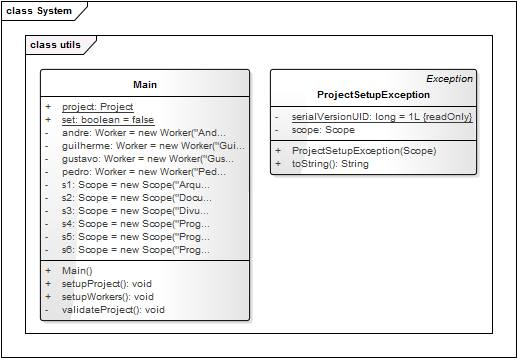
\includegraphics[scale=0.4]{uml4.png}
	\caption{Pacote responsável pela criação dos projetos}
\end{figure}
\begin{figure}
	\centering
	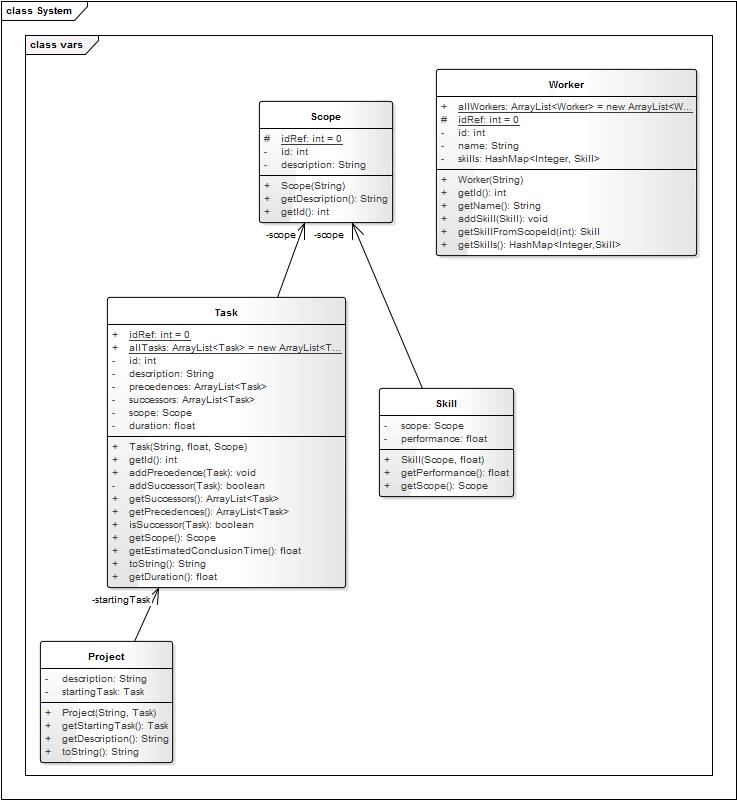
\includegraphics[scale=0.4]{uml5.png}
	\caption{Pacote com as variaveis de estudo}
\end{figure}
\paragraph{}

\newpage
\newpage
%%%%%%%%%%%%%%%%%%%%%%%%%%
\section{Experiências}
\subsection{Algoritmos Genéticos}
De modo a padronizar os resultados, avalariaremos o desempenho dos Algoritmos Genéticos com os seguintes parametros-base:
\begin{itemize}
	\item \textbf{Numero de cromossomas:} 50
	\item \textbf{Numero de geraçoes:} 100
	\item \textbf{Probabilidade de Mutação:} 0.01
	\item \textbf{Cortes por Crossover:} 2
	\item \textbf{Numero de Seleções:} 25
\end{itemize}
\paragraph{}
\begin{center}
	\begin{tabular}{ |l|l| }
		\hline
		\multicolumn{2}{|c|}{Resultados} \\
		\hline
		1º Ensaio & 6.889394 \\
		2º Ensaio & 6.283333 \\
		3º Ensaio & 6.392424 \\
		\textbf{Média} & 6.521717 \\
		\hline
	\end{tabular}
\end{center}

\paragraph{}
\subsubsection{Redução do numero de Cromossomas}
\begin{itemize}
	\item \textbf{Numero de cromossomas:} \textbf{25}
	\item \textbf{Numero de geraçoes:} 100
	\item \textbf{Probabilidade de Mutação:} 0.01
	\item \textbf{Cortes por Crossover:} 2
	\item \textbf{Numero de Seleções:} 12 (alteração proporcional)
\end{itemize}
\paragraph{}
\begin{center}
	\begin{tabular}{ |l|l| }
		\hline
		\multicolumn{2}{|c|}{Resultados} \\
		\hline
		1º Ensaio & 6.586363 \\
		2º Ensaio & 6.675252 \\
		3º Ensaio & 7.192424 \\
		\textbf{Média} & 6.818013 \\
		\hline
	\end{tabular}
\end{center}

\newpage
\subsubsection{Redução do numero de Gerações}
\begin{itemize}
	\item \textbf{Numero de cromossomas:} 50
	\item \textbf{Numero de geraçoes:} \textbf{50}
	\item \textbf{Probabilidade de Mutação:} 0.01
	\item \textbf{Cortes por Crossover:} 2
	\item \textbf{Numero de Seleções:} 25
\end{itemize}
\paragraph{}
\begin{center}
	\begin{tabular}{ |l|l| }
		\hline
		\multicolumn{2}{|c|}{Resultados} \\
		\hline
		1º Ensaio & 7.192424 \\
		2º Ensaio & 7.067965 \\
		3º Ensaio & 7.192424 \\
		\textbf{Média} & 7.150938 \\
		\hline
	\end{tabular}
\end{center}

\paragraph{}
\subsubsection{Aumento da probabilidade de Mutação}
\begin{itemize}
	\item \textbf{Numero de cromossomas:} 50
	\item \textbf{Numero de geraçoes:} 100
	\item \textbf{Probabilidade de Mutação:} \textbf{0.1}
	\item \textbf{Cortes por Crossover:} 2
	\item \textbf{Numero de Seleções:} 25
\end{itemize}
\paragraph{}
\begin{center}
	\begin{tabular}{ |l|l| }
		\hline
		\multicolumn{2}{|c|}{Resultados} \\
		\hline
		1º Ensaio & 6.889394 \\
		2º Ensaio & 6.089394 \\
		3º Ensaio & 6.889394 \\
		\textbf{Média} & 6.622727 \\
		\hline
	\end{tabular}
\end{center}

\newpage
\subsubsection{Aumento dos cortes por Crossover}
\begin{itemize}
	\item \textbf{Numero de cromossomas:} 50
	\item \textbf{Numero de geraçoes:} 100
	\item \textbf{Probabilidade de Mutação:} 0.01
	\item \textbf{Cortes por Crossover:} \textbf{4}
	\item \textbf{Numero de Seleções:} 25
\end{itemize}
\paragraph{}
\begin{center}
	\begin{tabular}{ |l|l| }
		\hline
		\multicolumn{2}{|c|}{Resultados} \\
		\hline
		1º Ensaio & 7.061616 \\
		2º Ensaio & 6.372222 \\
		3º Ensaio & 6.978283 \\
		\textbf{Média} & 6.804040 \\
		\hline
	\end{tabular}
\end{center}

\paragraph{}
\subsubsection{Diminuição das seleções por geração}
\begin{itemize}
	\item \textbf{Numero de cromossomas:} 50
	\item \textbf{Numero de geraçoes:} 100
	\item \textbf{Probabilidade de Mutação:} 0.01
	\item \textbf{Cortes por Crossover:} 2
	\item \textbf{Numero de Seleções:} \textbf{0}
\end{itemize}
\paragraph{}
\begin{center}
	\begin{tabular}{ |l|l| }
		\hline
		\multicolumn{2}{|c|}{Resultados} \\
		\hline
		1º Ensaio & 9.676282 \\
		2º Ensaio & 10.202076 \\
		3º Ensaio & 10.288235 \\
		\textbf{Média} & 10.062197 \\
		\hline
	\end{tabular}
\end{center}

\newpage
\subsection{Arrefecimento Simulado}
De modo a padronizar os resultados, avalariaremos o desempenho do Arrefecimento Simulado com os seguintes parametros-base:
\begin{itemize}
	\item \textbf{Temperatura:} 5000
	\item \textbf{Rácio de arrefecimento:} 0.9
\end{itemize}
\paragraph{}
\begin{center}
	\begin{tabular}{ |l|l| }
		\hline
		\multicolumn{2}{|c|}{Resultados} \\
		\hline
		1º Ensaio & 7.874739 \\
		2º Ensaio & 8.292819 \\
		3º Ensaio & 8.358585 \\
		\textbf{Média} & 8.175381 \\
		\hline
	\end{tabular}
\end{center}

\paragraph{}
\subsubsection{Aumento da Temperatura}
\begin{itemize}
	\item \textbf{Temperatura:} \textbf{10000}
	\item \textbf{Rácio de arrefecimento:} 0.9
\end{itemize}
\paragraph{}
\begin{center}
	\begin{tabular}{ |l|l| }
		\hline
		\multicolumn{2}{|c|}{Resultados} \\
		\hline
		1º Ensaio & 8.058585 \\
		2º Ensaio & 7.831871 \\
		3º Ensaio & 8.281203 \\
		\textbf{Média} & 8.057220 \\
		\hline
	\end{tabular}
\end{center}

\paragraph{}
\subsubsection{Diminuição do Rácio de arrefecimento}
\begin{itemize}
	\item \textbf{Temperatura:} 5000
	\item \textbf{Rácio de arrefecimento:} \textbf{0.99}
\end{itemize}
\paragraph{}
\begin{center}
	\begin{tabular}{ |l|l| }
		\hline
		\multicolumn{2}{|c|}{Resultados} \\
		\hline
		1º Ensaio & 7.412679 \\
		2º Ensaio & 7.864551 \\
		3º Ensaio & 7.443122 \\
		\textbf{Média} & 7.573450 \\
		\hline
	\end{tabular}
\end{center}

\newpage
%%%%%%%%%%%%%%%%%%%%%%%%%%
\section{Conclusões}
Relativamente ao trabalho desenvolvido, consideramos que a aplicação de algoritmos evolutivos ao planeamento de projetos pode-se tornar bastante eficiente para obtenção de uma solução eficaz.
\paragraph{}
Pelos testes realizados, podemos ver que é possível manipular o tipo de resultados que se pretendem, quer nos algoritmos genéticos (aumento do numero de cromossomas, de geraçoes ou seleções, por exemplo), quer no algoritmo de arrefecimento simulado (aumento da temperatura e diminuição do racio de arrefecimento), para obtenção de soluções otimizadas.
\paragraph{}
Realçamos ainda que, embora tenhamos testado a variação de todas variaveis possiveis, os resultados obtidos não são muito constrastantes, devido ao exemplo de projeto relativamente simples que estruturamos, para teste.
\paragraph{}
Consideramos este, um ótimo e interessante projeto, que permitiu a aplicação de conhecimentos de outras (biologia e metalurgia) à conceção de algoritmos consideravelmente eficazes para problemas como este.

\section{Melhoramentos}
Como melhorias ao projeto, focar-nos-iamos à criação de uma interface de utilizador mais completa, que permitisse a criação de um projeto e trabalhadores e capaz de fornecer estatísticas completas de forma clara e conclusiva.

\clearpage
\addcontentsline{toc}{section}{Bibliografia}
\renewcommand\refname{Bibliografia}
\bibliographystyle{plain}
\bibliography{myrefs}


\end{document}
